\section{Чем больше звуков, тем лучше? Аккорды}
\label{ch:harmony:chords}

Из раздела \ref{ch:harmony:interval} вы узнали, что \emph{интервал} для физиков --- это \emph{мера расстояния} между двумя звуками, а для лириков --- это \emph{два звука}, сыгранных одновременно или друг за другом.

Аккорд же --- понятие целиком лирическое.

\begin{Definition}[Аккорд]
    \emph{Аккорд} --- это три или более музыкальных звука, извлеченных (звучащих) одновременно.
\end{Definition}

Видели ведь, наверное, как играют <<боем>>? Правая рука ходит вверх-вниз, и ритмично бьет по всем струнам одним или несколькими пальцами. Говорить о том, что звуки извлекаются одновременно не приходится --- струны задеваются одна за другой, но так как это происходит достаточно быстро, то \emph{звучат} они некоторое время все вместе и мы слышим \emph{аккорд}.

Какие же звуки должны входить в аккорд, чтобы он звучал гармонично? Точно не любые. Есть ли правила построения аккордов?

Да, система аккордов сложилась и давно устоялась. Она определяет интервальную структуру аккордов и правила их именования, а в её основе лежат мажорный и минорный лады. Во всем множестве аккордов ярко выделяются две большие группы: мажорные (веселые) и минорные (грустные).

\begin{figure}[!ht]
    \centering
    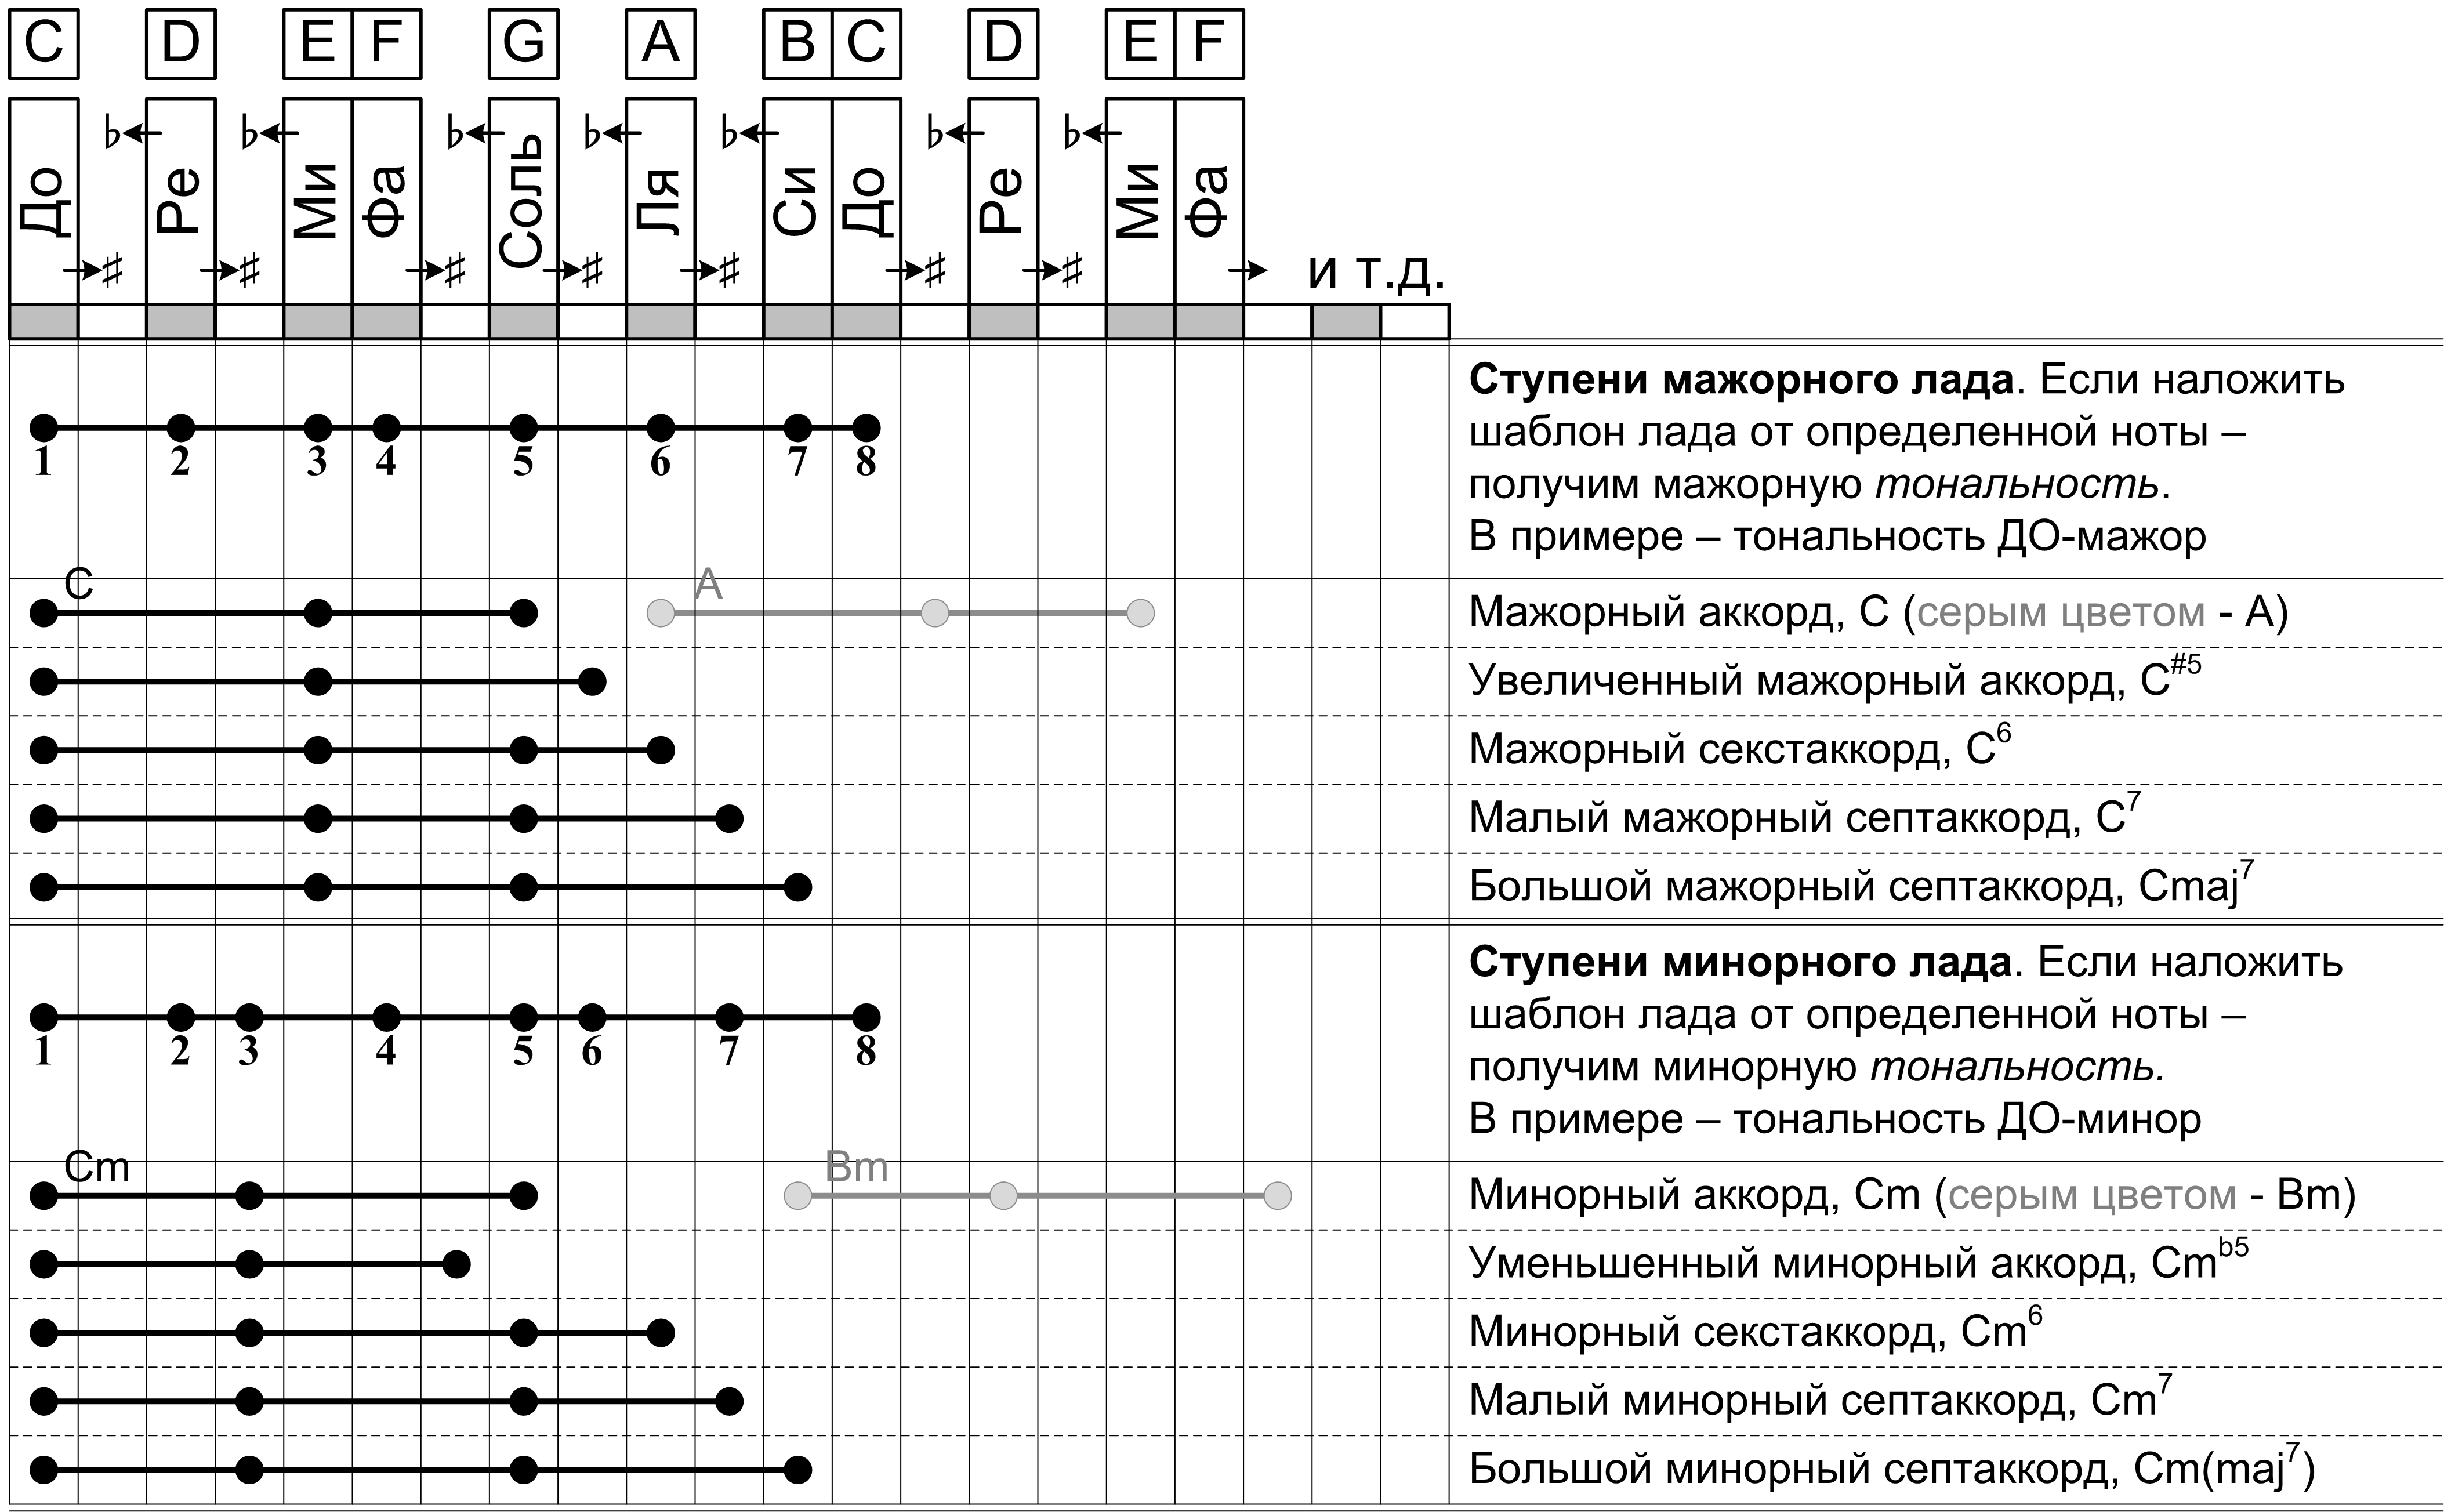
\includegraphics[width=\textwidth]{fig/chords/structure} 
    \caption{Интервальная структура некоторых аккордов}\label{fig:harmony:chords:structure}
\end{figure} 

Например, давайте рассмотрим интервальню структуру простого мажорного аккорда. Взгляните на рисунок \ref{fig:harmony:chords:structure}. В мажорный аккорд входят три музыкальных звука, на которые попадают соответственно первая, третья и пятая ступени мажорного лада. Первый, самый низкий, звук аккорда называется <<основным тоном>>\footnote{В западной терминологии основной тон аккорда называют root. Корень, источник. Все чаще и Русские люди называют основной тон <<корнем>> аккорда. А некоторые уважаемые люди (\cite{url:pimalive}) даже \emph{тоникой} аккорда!} аккорда. Второй звук будет отстоять от певого на 4 полутона, а третий от второго --- на 3 полутона. Интервальная структура мажорного аккорда:
\[
    \texttt{0-4-3}.
\]

Основной тон аккорда --- нота, от которой строится аккорд, определяет его название. Допустим, мы откладываем шаблон мажорого аккорда от ноты ДО (С). Получившееся трезвучие будет называться <<ДО-мажор>>, и в его состав войдут ноты: 
\[
    \text{ДО}\xrightarrow{4}
    \text{МИ}\xrightarrow{3}
    \text{СОЛЬ}
\]

Домисолька! Это не только название известного деткого музыкального театра города Москвы, но и веселый (мажорный) аккордик от ноты ДО! 

Аккорды принято обзначать в более короткой нотации. Так например, чтобы обозначить мажорный аккорд, просто используют латинское обозначение ноты основного тона. Домисолька будет обозначена кратко: <<C>>. А <<ЛЯ-мажор>>, в который входят ноты (см. рисунок \ref{fig:harmony:chords:structure}) ЛЯ(A), ДО-диез (C\#), МИ(E) будет обозначен как <<A>>.

Приведем краткий справочник обозначений и интервальных структур наиболее популярных типов аккордов с жалкими попытками найти логику в обозначениях (не забывайте поглядывать на рисунок \ref{fig:harmony:chords:structure}).

\begin{itemize}
    \item Мажорный аккорд. 
    \item Увеличенный мажорный аккорд. 
    \item Мажорный секстаккорд.
    \item Малый мажорный септаккорд.
    \item Большой мажорный септаккорд.
    
    \item Минорный аккорд.
    \item Уменьшенный минорный аккорд.
    \item Минорный секстаккорд.
    \item Малый минорный септаккорд.
    \item Большой минорный септаккорд.
\end{itemize}

Стоит отметить, что 
% TODO: надстройка и альтерация (знаки алтерации бемоль/диез)

% TODO: струн шесть - звука три
% пример аппликатурного бокса
%   построение аккорда в первой позиции
%   кошерные и некошерные аккорды не задеваем шестую!

% аппликатуры простейших аккордов, которые можно унести с баррэ в любое место грифа.


